\section{Comunicação} % (fold)
\label{sec:comunicação2}

	Com o objetivo de detalhar com maior clareza a implementação do sistema de comunicação do projeto, optou-se por utilizar a estratégia \textit{bottom-up}, apresentando toda a especificação técnica dos equipamentos de \textit{hardware} utilizados na solução,seguido da específicação em nível de \textit{Software}.

	\subsection{Hardware} % (fold)
	\label{sub:hardware}
		Um dos requisitos mais críticos do projeto é o da comunicação entre a base e o robô, pois todas as informações colatadas pelo robô são enviadas para a base realizar o processamento, já que a base possui um poder de processamento muito superior ao do próprio robô.

		A implementação do sistema com os \textit{hardwares} especificados na sessão \ref{sub:Hardwar_para_Comunicação} é apresentada na figura \ref{img:hardware_comunicação}.(REFAZER A FIGURA!)

		\begin{figure}[H]                                                           
      		\centering                    
      		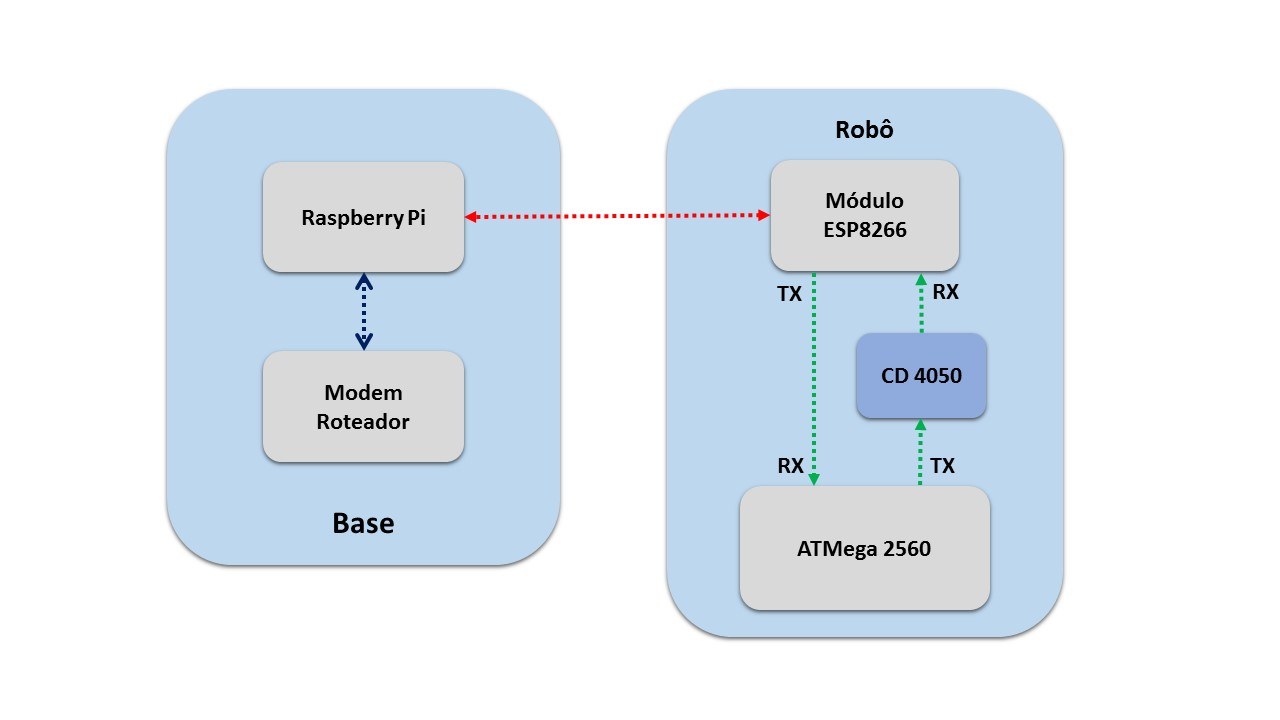
\includegraphics[scale=0.5]{figuras/Hardware_Comunicacao.jpg}               
      		\caption{Esquemático do hardware implementado para realizar a comunicação entre os microprocessadores.}    
      		\label{img:hardware_comunicação}                                            
    	\end{figure}

    	O sistema projetado para a base consiste em um modem roteador conectado a \textit{raspberry pi}, essa conexão é feita por meio de um cabo \textit{ethernet} e dessa forma o sistema é capaz de gerar uma subrede que deve ser acessada pelo robô e pelo usuário quando necessário. A seta vermelha na figura \ref{img:hardware_comunicação} representa essa comunicação entre o robô e a base que é feita via \textit{WiFi} utilizando o protocolo TCP/IP.

    	Para o robô foi necessário realizar alguns ajustes no projeto inicial que não contemplava o CI CD4050, ao consultar o datasheet do módulo ESP8266 foi constatado que o mesmo trabalha com tensões máximas de ate 3.3V e o controlador utilizado no robô gera sinais com ate 5V, a solução encontrada para resolver esse problema foi utilizar o CI CD4050, que consiste em um buffer não inversor que foi utilizado nesse contexto para converter o nível lógico alto de 5V para 3.3V, a figura \ref{img:datasheet_cd4050} mostra o esquemático interno do CI.

    	\begin{figure}[H]                                                           
      		\centering                    
      		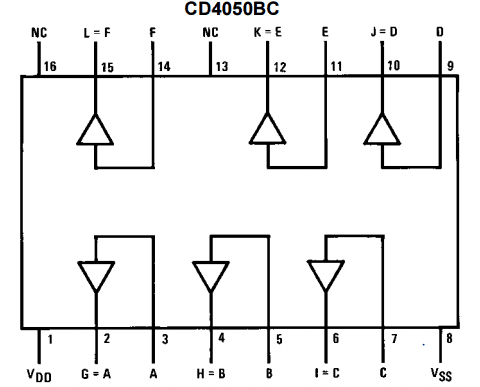
\includegraphics[scale=0.4]{figuras/cd4050.png}               
      		\caption{Esquemático interno do CD4050.(\href{http://www.embarcados.com.br/esp8266-com-arduino/}{Embarcados}})    
      		\label{img:datasheet_cd4050}                                            
    	\end{figure}

    	Por falha de observação, durante a primeira tentativa de montagem desse sistema, acidentalmente foi inserido no RX do módulo uma tensão de 5V, como mencionado anteriormente o módulo trabalha com tensões máximas de 3.3V o que resultou na queima do RX do componente impossibilitando a comunicação serial entre o módulo e o microprocessador, como solução foi adquirido outro módulo igual para continuar o processo de montagem, porem o módulo comprado apresentou falhas na sua inicialização de forma que não foi possível configura-lo da forma desejada, então como última solução foi adquirido um kit de desenvolvimento que garante a correta alimentação exigida pelo ESP8266 facilitando a utilização do mesmo, este foi devidamente configurado de acordo com o projeto e posteriormente será incorporado ao protótipo do projeto, a figura \ref{img:kit_desenvolvimento} apresenta o kit adquirido.

    	\begin{figure}[H]                                                           
      		\centering                    
      		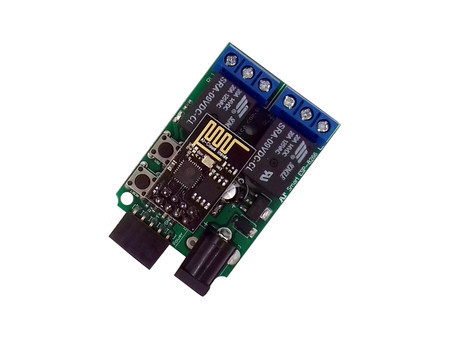
\includegraphics[scale=0.5]{figuras/kit_desenvolvimento.jpg}               
      		\caption{Kit de desenvolvimento ESP8266 \textit{WiFi} 802.11 B/g/n.(\href{http://www.afeletronica.com.br/pd-31421a-esp8266-wifi-802-11-b-g-n-kit-desenvolvimento.html}{AF Eletrônica}})    
      		\label{img:kit_desenvolvimento}                                            
    	\end{figure}

    	Este kit necessita de uma alimentação de 9V/1A, sua alimentação será realizada pela bateria do robô e somente os pinos correspondente ao RX e ao TX serão utilizados pelo microprocessador para realizar a comunicação serial. Essa comunicação serial é representada na figura \ref{img:hardware_comunicação} pelas setas verdes.
	% subsection hardware (end)

	\subsection{Software} % (fold)
	\label{sub:software}
		
		Para realização da comunicação, está sendo utilizado o protocolo de comunicação TCP, enviando e recebendo dados a partir de uma conexão via \textit{sockets} em uma rede criada por um roteador fixo na base. A estratégia de comunicação foi pensada com o objetivo de possibilitar o funcionamento de diversos robôs em uma residência, utilizando a mesma base de processamento. Desse modo, o servidor executado na \textit{raspberry}, em C, aguarda por conexões que podem ser feitas por qualquer cliente que deseje conectar na porta correta (definida neste projeto como 8090).

		Ao identificar uma conexão, uma \textit{thread} é gerada para tratar aquela conexão, entrando em um loop infinito até que o cliente ou o servidor opte por encerrar a conexão. Toda a comunicação realizada entre o robô e a base é feita a partir desta \textit{thread}.

		Quando a \textit{thread} para tratamento da conexão é lançada, a mesma faz a criação de uma nova \textit{thread} que executará paralelamente a ela, que será responsável por enviar comandos ao robô. Ou seja, são criadas duas \textit{threads} para tratar uma mesma conexão, uma \textit{thread} responsável por obter os dados enviados pelo robô e outra responsável por processar estes dados e enviar comandos ao robô.

		Como apenas um canal de comunicação é utilizado, foi necessário utilizar um protocolo que define os padrões de comunicação entre o servidor e o robô. Este protocolo envolve duas partes, onde a primeira representa o \textit{tipo de informação} e a segunda parte representa a \textit{informação} em si. A tabela \ref{tab:protocolo_comunicacao1} apresenta os padrões já definidos e implementados no sistema em relação a comunicação do servidor para o robô.

		\begin{table}[H]
		\centering
		\caption{Padrões de comunicação - Servidor-Robô}
		\label{tab:protocolo_comunicacao1}
		\begin{tabular}{|c|c|}
		\hline
		\multicolumn{2}{|c|}{\textbf{Servidor -\textgreater Robô}} \\ \hline
		\textbf{Padrão}           & \textbf{Descrição}             \\ \hline
		\textit{L 90}             & Virar 90º a esquerda           \\ \hline
		\textit{R 90}                      & Virar 90º a direita            \\ \hline
		\textit{F 10}                      & Andar 10cm a frente            \\ \hline
		\textit{S}                         & Stop                           \\ \hline
		\textit{R}                & Run                            \\ \hline
		\textit{B 10}             & Andar 10cm para trás           \\ \hline
		\textit{B}                & Voltar para base               \\ \hline
		\end{tabular}
		\end{table}

		Já na tabela \ref{tab:protocolo_comunicacao2} estão apresentados os padrões referentes a comunicação do robô para o servidor.

		\begin{table}[H]
		\centering
		\caption{Padrões de comunicação - Robô-Servidor}
		\label{tab:protocolo_comunicacao2}
		\begin{tabular}{|c|c|}
		\hline
		\multicolumn{2}{|c|}{\textbf{Robô -\textgreater Servidor}} \\ \hline
		\textbf{Padrão}        & \textbf{Descrição}                \\ \hline
		\textit{L 90}          & Distância esquerda: 90cm          \\ \hline
		\textit{R 90}                   & Distância direita: 90cm           \\ \hline
		\textit{F 10}                   & Distancia frente: 10cm            \\ \hline
		\textit{B 10}                   & Distancia ré: 10cm            \\ \hline
		\textit{A 45}                   & Bateria 45\%                      \\ \hline
		\textit{P 42}          & Potência do sinal wifi: 42        \\ \hline
		\end{tabular}
		\end{table}

		Com a utilização destes padrões de comunicação, ficou fácil implementar um \textit{porteiro} de cada lado que seja capaz de distribuir as informações para seus respectivos contextos. Esta é a estratégia básica de comunicação entre os dois módulos, mas para isso, uma estrutura foi inicialmente desenvolvida.

		Para realização da comunicação entre os módulos e cliente, faz-se necessário um sistema de autenticação na rede e no sistema de gerenciamento de limpezas. Para isso, foi levantada uma base LDAP de autenticação, utilizando o protocolo RADIUS para conexão na rede. O sistema de gerenciamento de limpezas pode cadastrar novos usuários, incluindo-os na base LDAP, para que o mesmo cadastro realizado no sistema possa ser utilizado para login na rede.

		A arquitetura do sistema, apresentada na seção \ref{sub:arquitetura} registra de maneira clara o funcionamento do sistema de comunicação do projeto. 

	% subsection software (end)
% section comunicação (end)